\chapter{Introdução} \label{chap:intro}

Este trabalho surge no contexto do desenvolvimento do projeto realizado no âmbito na Unidade Curricular Dissertação, pertencente ao plano de estudos do Mestrado Integrado em Engenharia Eletrotécnica de Computadores. Nesta secção é feita uma análise introdutória do projeto, quer do ponto de vista geral em que este se enquadra, quer do ponto de vista motivacional do mesmo. Por fim, é feita uma descrição do problema dos objetivos do mesmo e da estrutura desta dissertação. 


\section{Enquadramento Geral} \label{sec:context}
Ao longo das últimas décadas a sociedade tem vindo a tornar-se cada vez mais dependente das comunicações com e sem fios, não só em termos empresariais, mas também pessoais. Esta tendência tem vindo a vincar-se recentemente com a crescente utilização de \textit{tablets} e \textit{smartphones}, tornando os recursos atuais incapazes de responder a tal procura. E cada vez mais esta exigência irá aumentar prevendo-se a necessidade de ligações na ordem das centenas de \SI{}{\giga\bit\per\second} no ano de 2020, essencialmente para comunicações a curta distância. Daqui conclui-se que os recursos que existem atualmente não são capazes de responder a esta necessidade crescente de comunicações de alto débito, e como tal é necessário urgentemente o desenvolvimento de tecnologias não só capazes de satisfazer esta procura, mas ao mesmo tempo que o façam de forma eficiente em termos energéticos e financeiros. Neste contexto enquadra-se o projeto \textit{iBrow} (\textit{Innovative ultra-BROadband ubiquitous Wireless communications through terahertz transceivers}), o qual está a ser parcialmente desenvolvido pela equipa de investigação de tecnologias óticas e eletrónicas do INESC-TEC (Instituto de Nacional de Engenharia de Sistema e Computadores Tecnologias e Ciências), que vem responder a esta necessidade de uma forma eficiente.

O projeto \textit{iBrow} vem propor o desenvolvimento de uma tecnologia capaz de responder a esta necessidade de comunicações de alto débito através de uma utilização eficaz do espetro de frequências promovendo a utilização de bandas de frequência mais altas, desde \SI{60}{\giga\hertz}  até \SI{1}{\tera\hertz}. Para além disso vem também propor uma metodologia, que pela primeira vez permite um baixo custo de manufaturação de transcetores capazes de atingir altos débitos de transmissão para que possam ser perfeitamente integrados em redes de comunicações ótica de grande velocidade.
 
Todo este crescente de consumo por parte dos utilizadores de novas e cada vez mais tecnologias não se verifica apenas na necessidade de aumento de largura de banda para as comunicações, mas existe também uma necessidade extrema da existência de interfaces digitais de vídeo e som que não só sejam capazes de fazer chegar ao utilizador sinais de alto débito, mas que ao mesmo tempo o façam de maneira segura no sentido de proteger eventuais cópias não autorizadas. Assim sendo, o desenvolvimento de um conversor HDMI \textit{(High Definition Multimedia Interface}) de alto débito enquadra-se perfeitamente nesta necessidade sendo que é a interface de vídeo e áudio \textit{standard} e que implementa o protocolo HDCP (\textit{High-bandwith Digital Content Protection}) que protege a reprodução de sinais em dispositivos não autorizados.

Existem várias interfaces digitais que implementam o protocolo referido anteriormente, entre elas destacam-se \textit{DisplayPort}, DVI (\textit{Digital Visual Interface}) e HDMI. No entanto, devido ao tremendo sucesso que a interface HDMI obteve, de acordo com \textit{In-Stat} referido em \cite{R002} foram vendidos 5 milhões de exemplares em 2004, 17,4 milhões em 2005, 63 milhões em 2006 e 143 milhões em 2007, tornou-se a interface \textit{standard} para HDTV (\textit{High-Definition Television}), substituindo a interface DVI. Relativamente à interface \textit{DisplayPort}, esta é utilizada em vários equipamentos, mas principalmente no setor dos computadores e vem complementar o HDMI. Contudo, comparando as duas interfaces previamente referidas, o HDMI tem algumas vantagens no que toca à capacidade de transmitir sinais CEC (\textit{Consumer Electronics Control}) e a compatibilidade elétrica com o DVI. Mas o que destaca esta interface é a sua capacidade de transmissão dos sinais na sua largura de banda completa até 10 metros, enquanto que a \textit{DisplayPort} apenas o consegue transmitir até 3 metros.

Através da implementação dos objetivos propostos pela dissertação será possível implementar um conversor HDMI capaz de fazer transmitir sinais de alto débito, tornando mais eficiente este tipo de comunicações e ao mesmo tempo fazendo-o de forma segura, protegendo as cópias e reproduções não autorizadas dos sinais transmitidos.
 

\section{Motivação} \label{sec:goals}
Com a explosão que se fez sentir nos últimos anos na utilização do espetro de frequências, verifica-se que é necessário tornar a sua utilização mais eficiente no sentido de conseguir satisfazer a necessidade da sociedade de comunicar quase sem limites em termos de velocidade da comunicação em si. Promove-se assim uma nova abordagem do espetro de frequências, de maneira a que se possa utilizá-lo de uma forma mais eficaz.  
Ao longos dos anos tem-se vindo a verificar melhorias no que toca à eficiência espetral através do desenvolvimento e aplicação de algumas técnicas, tal como referido em \cite{R007}, como por exemplo o QAM (\textit{Quadrature Amplitude Modulation}) para modulação do sinal e também técnicas MIMO (\textit{Multiple Input Multiple Output}) nas entradas e saídas do sistema de comunicação. Verificou-se que o aproveitamento do espetro de facto melhorou, no entanto, estas técnicas não são suficientes para se conseguir atingir um débito de algumas dezenas ou centenas de \SI{}{\giga\bit\per\second}. Assim sendo, a solução passa por promover a utilização de bandas de frequência mais altas, contrariamente ao que se fez no passado.  

Por definição, considera-se a banda de ondas mm entre 60 a \SI{100}{\giga\hertz} e a banda THz entre \SI{100}{\giga\hertz} a \SI{1}{\tera\hertz}. Estas bandas do espetro de frequências são bandas cuja utilização no passado foi pouca ou até mesmo nenhuma, isto porque para conseguir explorar estas bandas são necessários componentes adequados à operação nas mesmas. Relativamente à banda de ondas mm, apesar de nos últimos anos terem sidos desenvolvidas e aplicadas técnicas que melhoram a eficiência espetral desta região, tal como referido anteriormente, a escassez da largura de banda limita o débito da ligação. Em \cite{R007} são referidas implementações realizadas no passado que conseguiram alcançar débitos até  \SI{100}{\giga\hertz} em ligações sem fios a uma distância de 1 metro com BER (\textit{Bit Error Ratio}) igual a \num{1e-3} recorrendo também à utilização de mais de um transmissor e recetor. Apesar de inovadores estes valores revelam-se insuficientes para o que se pretende alcançar. 

Quanto à região do espetro que corresponde a uma frequência superior a \SI{10}{\tera\hertz}, apesar da grande largura de banda disponível nesta região, existem várias limitações para a comunicação sem fios referidas em \cite{R005}. Destaca-se o facto do baixo balanço de potência possível para a transmissão devido aos limites de segurança dos olhos, os impactos atmosféricos na propagação do sinal (chuva, pó e poluição) e ainda o impacto da falta de alinhamento entre transmissores e recetores. Estas são algumas das razões que limitam a comunicação sem fios para frequências superiores a \SI{10}{\tera\hertz}.

Assim sendo, segundo \cite{R005}, torna-se evidente que a banda do espetro com maior potencial para a comunicação sem fios é a banda entre \SI{100}{\giga\hertz} e \SI{1}{\tera\hertz}, uma vez que não só oferece uma largura de banda bastante maior (desde \SI{}{\giga\hertz} até alguns  \SI{}{\tera\hertz}) comparativamente a outra bandas, mas também é uma região do espetro que não sofre muito devido às más condições atmosféricas. Para além disso, a utilização destas bandas de frequência altas acabará por aliviar o espetro relativamente à sua escassez e às suas limitações de capacidade. 

Tendo em conta esta nova abordagem do espetro, o projeto iBrow tem vindo a desenvolver metodologias que permitem a manufaturação de transcetores para operar a estas frequências de baixo custo, mas que ao mesmo tempo são capazes de atingir altos débitos, para que desta maneira sejam integrados em redes de comunicação com e sem fios de grande velocidade. Os transcetores de baixo custo propostos pelo projeto passam por utilizar díodos ressonantes de efeito túnel (RTD - \textit{Resonant Tunneling Diode}) com formatos de modulação simples e com interligação com fibra ótica. Assim, será possível satisfazer as necessidades previstas para 2020 de forma eficaz tanto em termos energéticos como financeiros.


A principal motivação do projeto proposto nesta dissertação passa por desenvolver um trabalho que possa demonstrar o potencial da tecnologia proposta pelo \textit{iBrow}, recorrendo à transmissão de vídeo em alta definição descomprimido pelos dispositivos propostos pelo projeto. Para efetuar a transmissão é utilizada a interface HDMI, que faz transmitir um sinal de alto débito para de seguida o mesmo sinal ser transmitido pelos transcetores propostos pelo projeto iBrow. Esta transmissão terá de ser realizada em série visto que estes mesmos transcetores apenas suportam transmissão de dados em série.

O HDMI é uma interface digital que transmite vídeo não comprimido e áudio que poderá ou não estar comprimido. Esta interface implementa vários protocolos entre quais se destaca o protocolo HDCP pois é o responsável pela prevenção de reproduções não autorizadas dos sinais a transmitir, o que é bastante importante hoje em dia dado os inúmeros consumidores que conseguem fazer cópias ilegais. Este protocolo faz uma verificação inicial antes de transmitir os dados encriptados no sentido de perceber se o dispositivo de destino é efetivamente um dispositivo autorizado para a reprodução de sinal. Esta é ainda uma interface que consegue transmitir sinais de alta definição e é ainda compatível com o DVI. Hoje em dia, esta é a interface \textit{standard} para HDTVs e tem diversas aplicações tais como câmaras digitais, discos \textit{Blu-ray} e leitores de DVD (\textit{Digital Video Disc}) de alta definição, computadores pessoais, \textit{tablets} e \textit{smartphones}.

Em suma, esta implementação torna-se bastante útil, uma vez que é capaz de abranger um vasto nível de aplicações acessíveis a todos os utilizadores, tanto em ambientes empresariais como pessoais.

%\section{Objetivos} \label{sec:struct}
%Este trabalho tem como principal objetivo a implementação de uma arquitetura de serialização e deserialização de um sinal HDMI, e que ao mesmo tempo faça o tratamento destes mesmos sinais para posterior envio e receção do sinal de alta velocidade em série. Como tal, será necessário utilizar um recurso que permita a implementação dessa mesma arquitetura versatilmente, por outras palavras, um recurso que permita eventuais reconfigurações da arquitetura desenvolvida e que ao mesmo tempo possua características que sejam úteis ao desenvolvimento do projeto.
%
%O projeto fará uso então de uma FPGA VC7203 Virtex-7 que possibilita a implementação de uma arquitetura adequada e que ao mesmo tempo possui entradas e saídas de alta velocidade que vão ajudar na ligação do sinal com os transcetores de alta velocidade. O protótipo desenvolvido em hardware reprogramável deve ser devidamente validado para que o sinal digital possa de seguida ser transmitido através de uma ligação por fibra ótica usando os RTDs desenvolvidos no projeto iBrow.

\section{Descrição do Problema e Objetivos} \label{sec:descrição_objetivos}

Este projeto tem como principal objetivo a implementação de uma arquitetura que permita a receção de dados HDMI, o seu tratamento e serialização para o seu posterior envio em alta velocidade. Para além disto, a arquitetura deve também receber os dados em série, fazer a sua conversão para paralelo e voltar a enviar para um dispositivo HDMI final.

\begin{figure}[h!]
	\begin{center}
		\leavevmode
		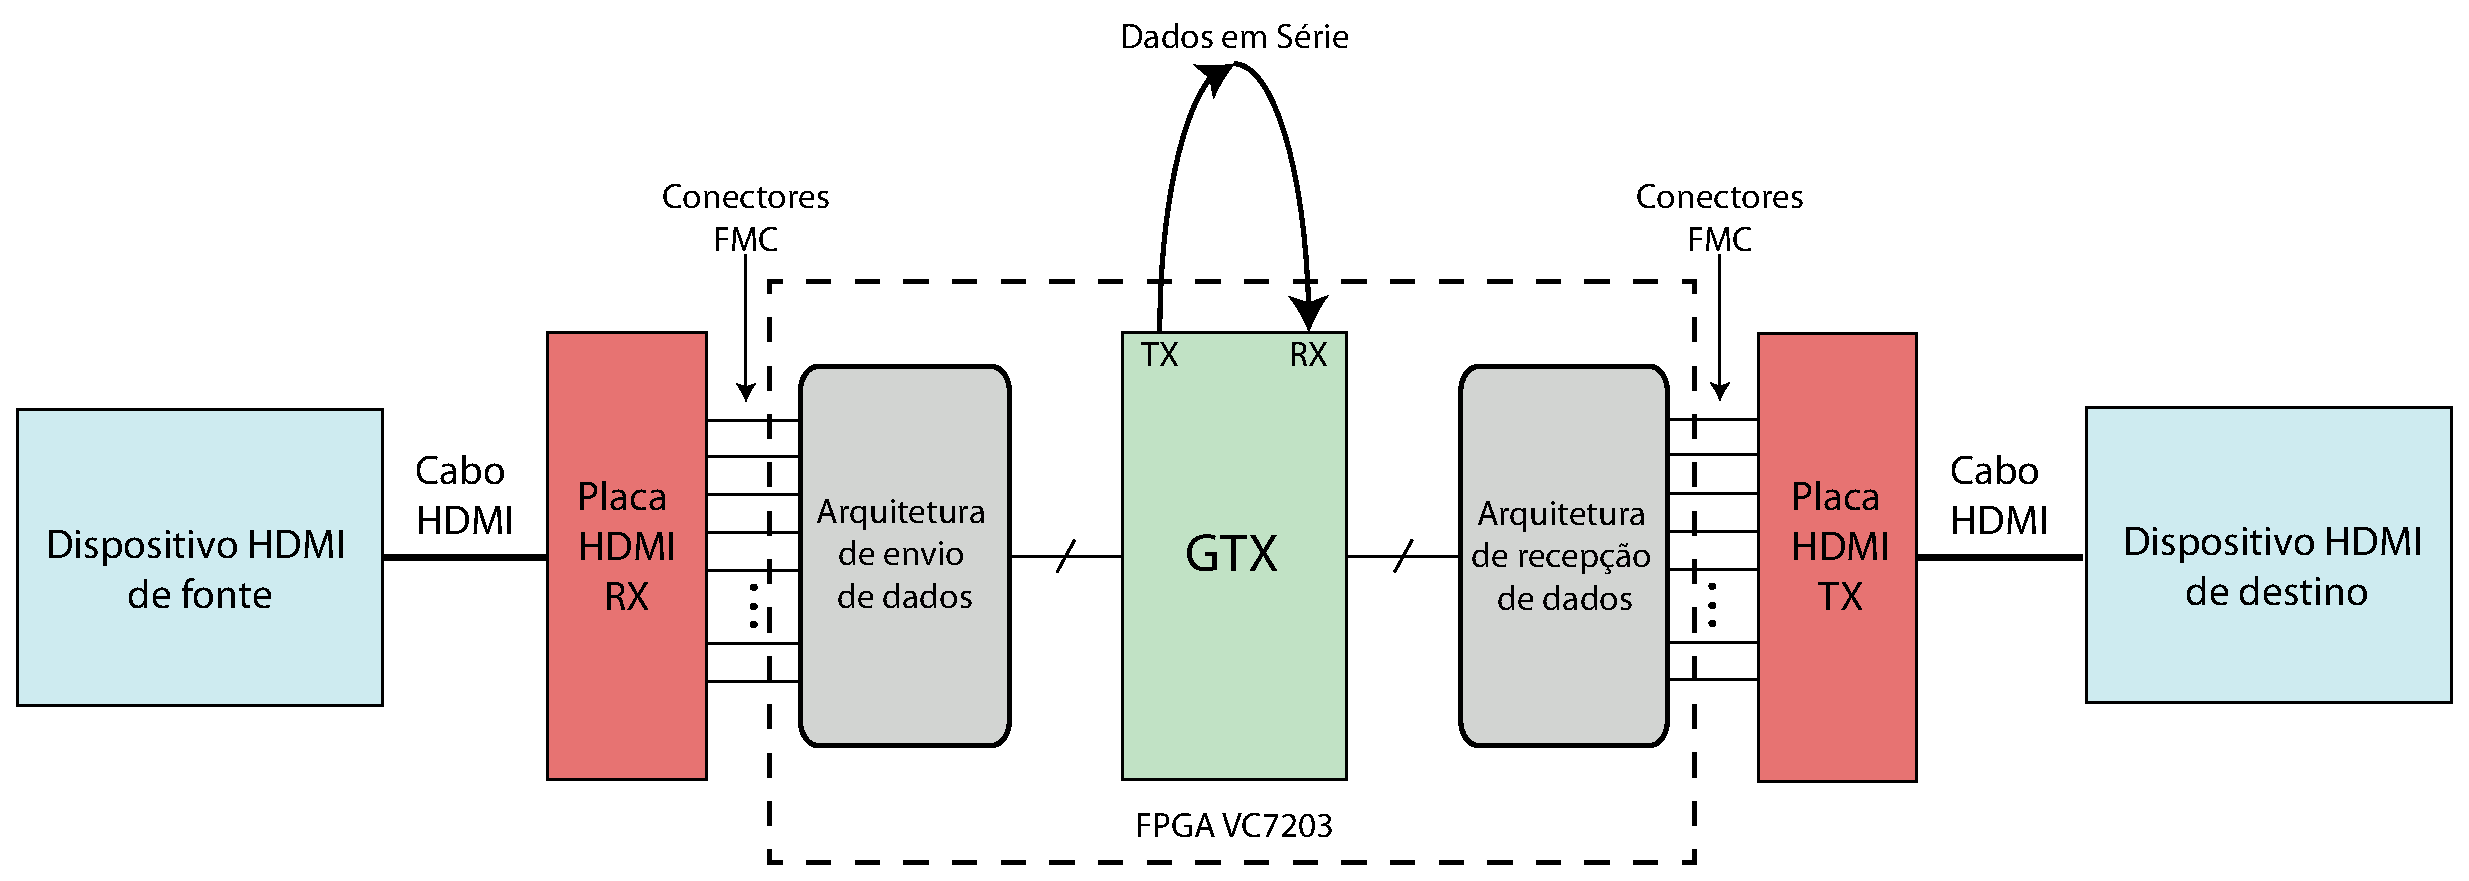
\includegraphics[width=1.0\textwidth]{diagrama_inicial}
		\caption{Diagrama geral do problema proposto}
		\label{fig:diagrama_inicial}
	\end{center}
\end{figure}

O projeto faz uso de uma FPGA (\textit{Field-Programmable Gate Array}) VC7203 (\textit{Virtex-7}) que possibilita a implementação de uma arquitetura adquada e ao mesmo tempo possui entradas e saídas de alta velocidade para testar a arquitetura desenvolvida. Para além disso, são também utilizadas umas placas HDMI que permitem enviar os dados em paralelo de um fonte HDMI para a FPGA VC7203 através dos conectores FMC (\textit{FPGA Mezzanine Cards}), e depois fazer o processo inverso, ou seja, enviar os dados em paralelo para a placa transmissora para que esta os transmita para o dispositivo final HDMI.

A figura \ref{fig:diagrama_inicial}  ilustra o diagrama geral do projeto a ser realizado. No sentido de simplificar o seu desenvolvimento, este foi dividido em duas partes:
\begin{enumerate}
	\item Conceção e desenvolvimento de arquiteturas que permitam comunicação entre dispositivos HDMI.
	\item Conceção e desenvolvimento de arquiteturas que permitem serialização de dados e deserialização dos mesmos.
\end{enumerate}

A primeira parte do projeto consiste em obter comunicações entre dois dispositivos HDMI utilizando para tal as placas HDMI disponíveis. A figura \ref{fig:1parte_projeto} ilustra um diagrama que descreve a primeira parte do projeto.
\begin{figure}[h!]
	\begin{center}
		\leavevmode
		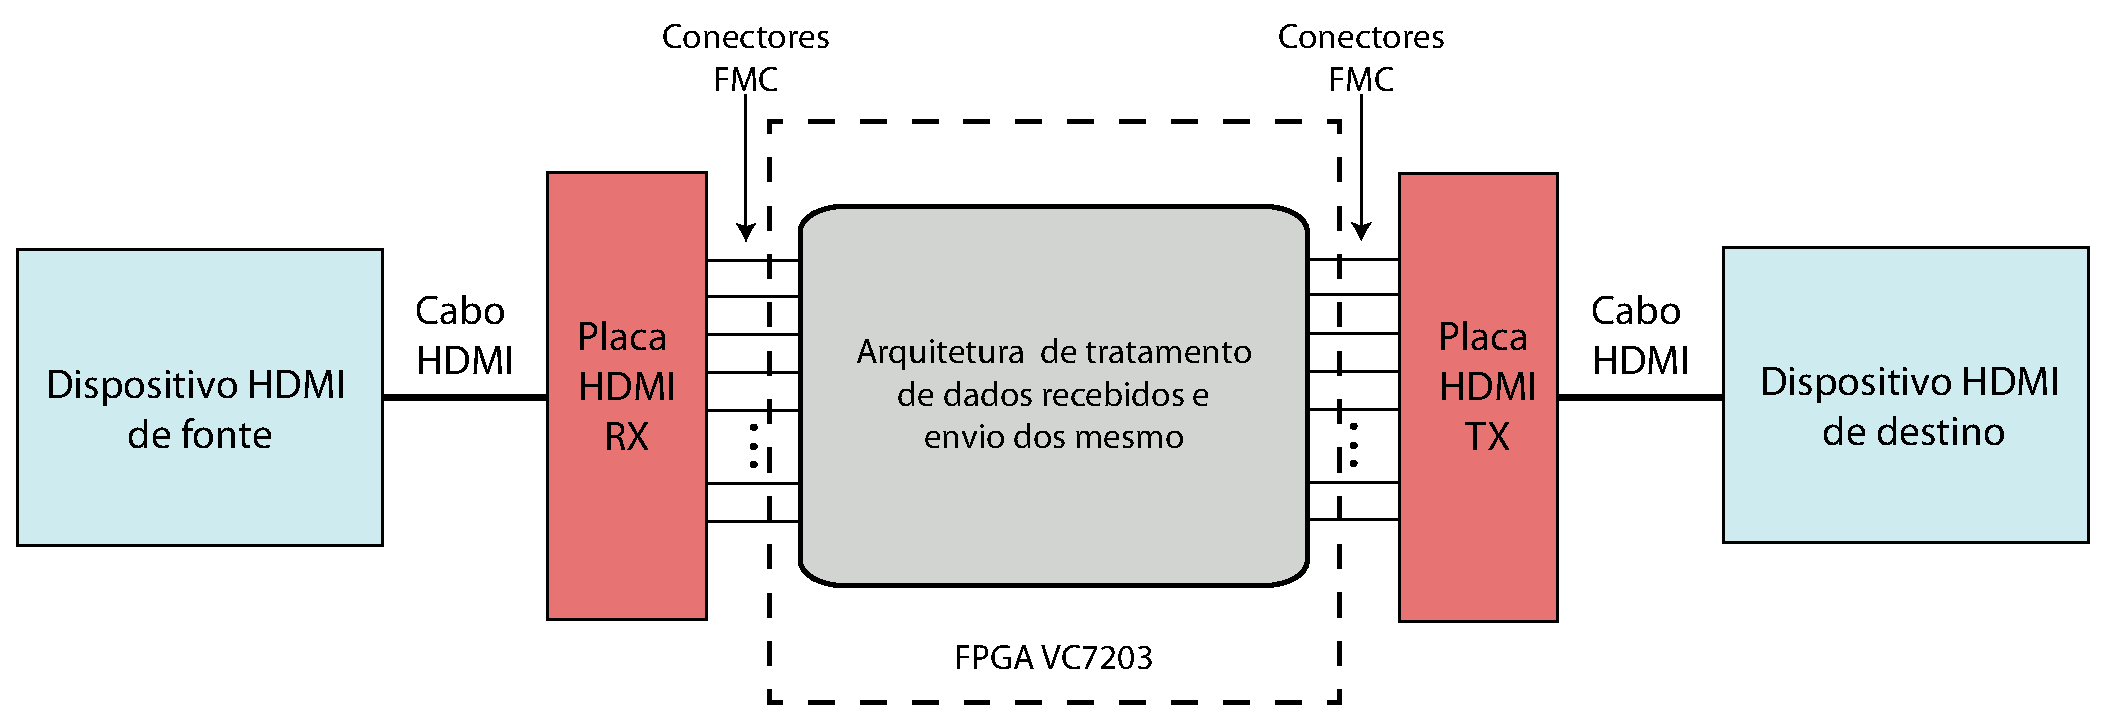
\includegraphics[width=1.0\textwidth]{1aparte}
		\caption{Diagrama geral da primeira parte do problema}
		\label{fig:1parte_projeto}
	\end{center}
\end{figure}

À placa HDMI recetora é ligado um sinal externo via cabo HDMI de uma fonte e de seguida essa mesma placa envia para a FPGA, através dos conectores FMC, os sinais de vídeo a serem transmitidos. Na FPGA VC7203 é desenvolvida uma arquitetura que permite o tratamento dos dados provenientes dos conectores FMC e de seguida, esses mesmo dados, são enviados para a placa HDMI transmissora de maneira a que esta os transmita para o dispositivo de destino.

A segunda parte do projeto consiste em desenvolver uma arquitetura na FPGA que permite serializar os dados recebidos enviá-los através das saídas de alta velocidade da mesma e voltar a recebê-los. A figura \ref{fig:2parte_projeto} ilustra o diagrama do trabalho a ser desenvolvido nesta fase.

\begin{figure}[h!]
	\begin{center}
		\leavevmode
		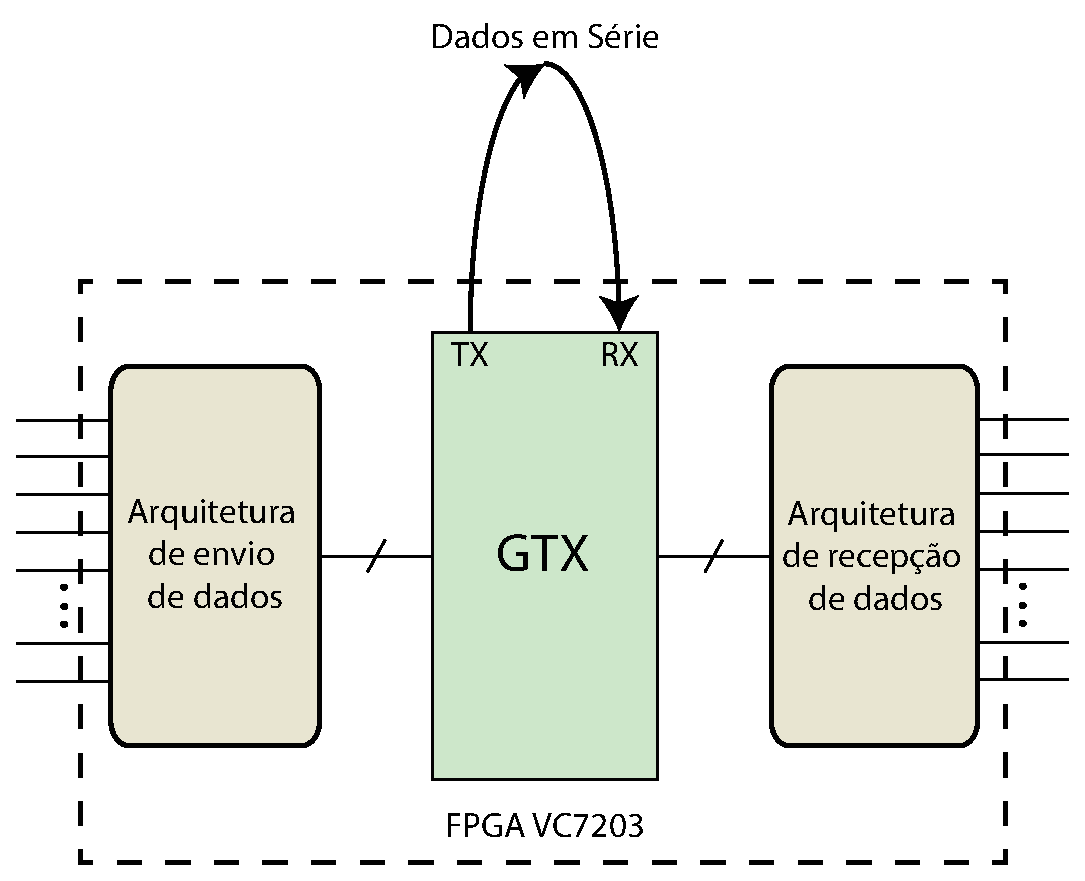
\includegraphics[width=0.7\textwidth]{2parte}
		\caption{Diagrama geral da segunda parte do problema}
		\label{fig:2parte_projeto}
	\end{center}
\end{figure}

Tal como ilustra a figura \ref{fig:2parte_projeto}, deve ser desenvolvida uma arquitetura que organize os dados em paralelo em tramas e de seguida os envie para os transcetores da FPGA que automaticamente fazem a sua serialização. Os dados em série são transmitidos por um cabo físico e recebidos nos transcetores onde são deserializados novamente. Por fim, as tramas são recebidas e processadas de modo a obter-se na saída os dados em paralelo tal como recebidos na entrada. Assim que as duas partes do projeto estejam concluídas obtém-se o objetivo final.

\section{Estrutura da Dissertação} \label{sec:struct}

Esta dissertação está organizada em vários capítulos que vão desde uma revisão bibliográfica do problema até à descrição da resposta ao mesmo. 
No capítulo \ref{chap:chap2} é feita uma revisão bibliográfica sobre os diversos aspetos que o problema apresenta, expondo também considerações de diversos autores sobre esses mesmos aspetos.  

No capítulo \ref{chap:chap3} é descrita toda a concepção e desenvolvimento das arquiteturas referentes à primeira parte do trabalho apresentado em \ref{sec:descrição_objetivos}. Todas estas são devidamente detalhadas e são ainda apresentados os principais resultados obtidos.

O capítulo \ref{chap:chap4} aborda todas as questões relativas à transmissão em série. Uma vez que existem transcetores disponíveis nos recursos utilizados, neste capítulo são apresentadas as arquiteturas dos mesmo e as características mais relevantes para o correto funcionamento do projeto em geral. No capítulo \ref{chap:chap5} são apresentas as arquiteturas desenvolvidas para se obter uma ligação em série, todas as suas características e ainda são explicadas as decisões tomadas quanto à escolha de determinados parâmetros.

O capítulo \ref{chap:concl} expõe as conclusões finais de todo o trabalho realizado e ainda aborda trabalho que pode futuramento ser realizado decorrente do que foi realizado até ao momento.

